\section{Updates and Hardforks [Procedure proposal]}

During normal operation of the blockchain certain updates or changes need to be made on the validator system. These updates can contain operating system updates, updates for any of the system components or updates to the chain specification. All these updates will be coordinated by EWF NetOps.
Short abstract of the full flow as shown in Figure ~\ref{fig:updateflow}.

\begin{enumerate}
    \item NetOps prepares the update and proposes it to GovOps
    \item GovOps decides on it
    \item NetOps splits active validators into waves
    \item NetOps will trigger the update process
    \item Nodes will report back success or failure of update
    \item When all waves are completed the update is finished
\end{enumerate}

Should a node not be able to finish the update the complete process for the entire system is reverted. The node can then be fixed manually by the affiliate in a given period of time or has to be removed from the validator set as it no longer updateable.

\begin{figure}[ht]
	\centering
    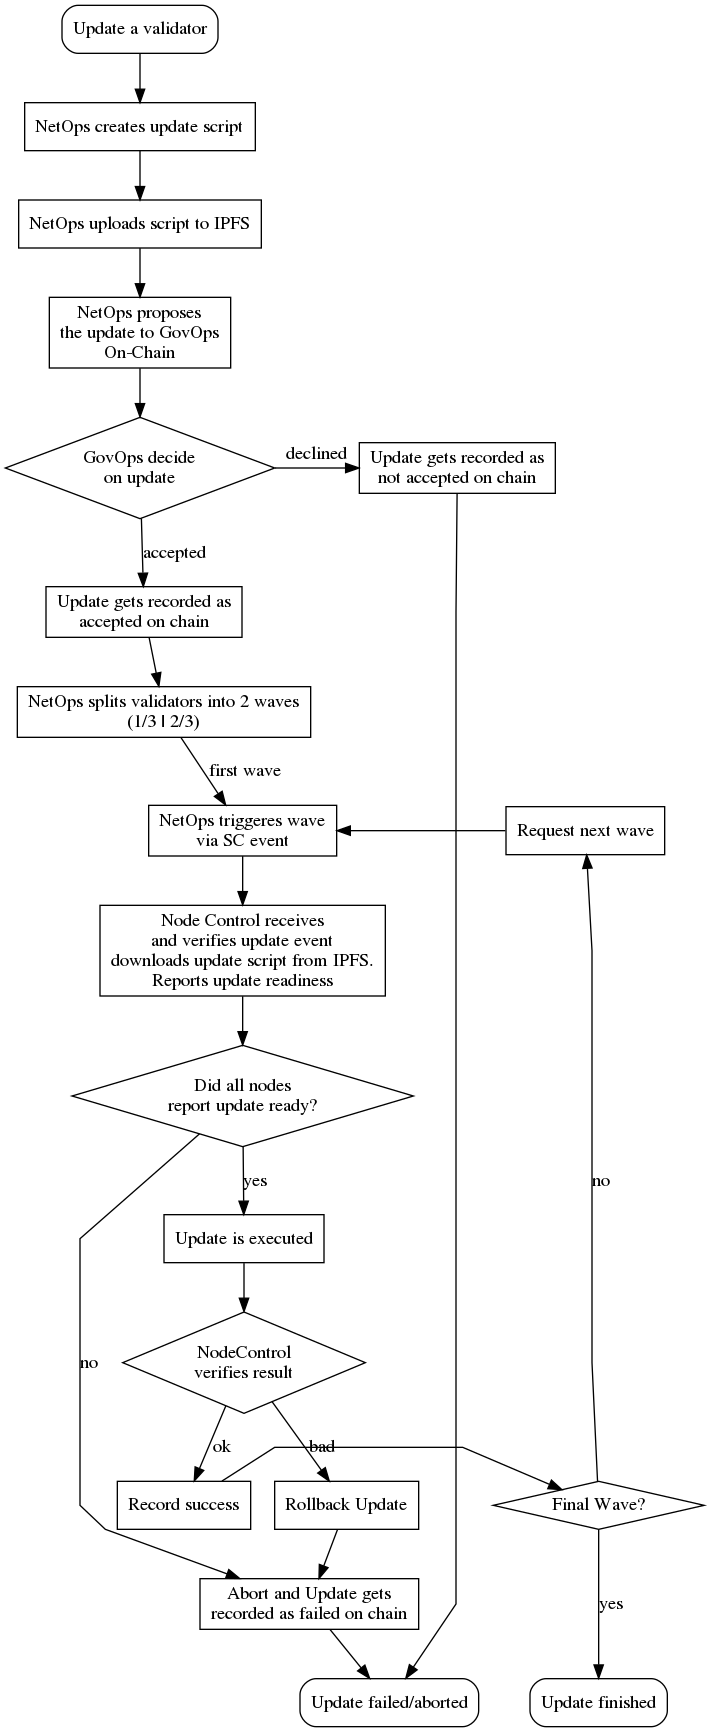
\includegraphics[width=\textwidth,height=\textheight,keepaspectratio]{./images/flow-update-validator.png}
	\caption{Update Flow}
	\label{fig:updateflow}
\end{figure}

Most updates will be executed automatically through NodeControl.

If the affiliate does not carry out the upgrade procedures during the time frame, NetOps will escalate the matter to GovOps which then will decide upon the removal of the authority node from the validator set.
